\documentclass[12pt]{article}
\usepackage{graphicx}

\title{Are consecutive annual mean temperatures in a given location
significantly correlated?}

\author{Ben Nouhan, bjn20@ic.ac.uk}

\date{\today}


\begin{document}
\maketitle

\section{Introduction}

The aim of this study was to determine whether temperatures in a 
This paper investigates whether temperatures of one year significantly
correlates with the next year for successive years, across years in a 
given location.

The null hypothesis states that temperatures of one year do not 
significantly correlate with the next year for successive years, across
years in a given location. The alternative hypothesis states that 
temperatures are correlated. Temperature data across multiple years in 
Key West, Florida is being investigated in this paper.

A significance level of less than 0.05 is required for the correlation to be
significant. However, temperature data between years are not independent, thus 
samples of randomly ordered temperature data is generated in order to calculate
the p-value.

\begin{figure}[hbt!]
\centering
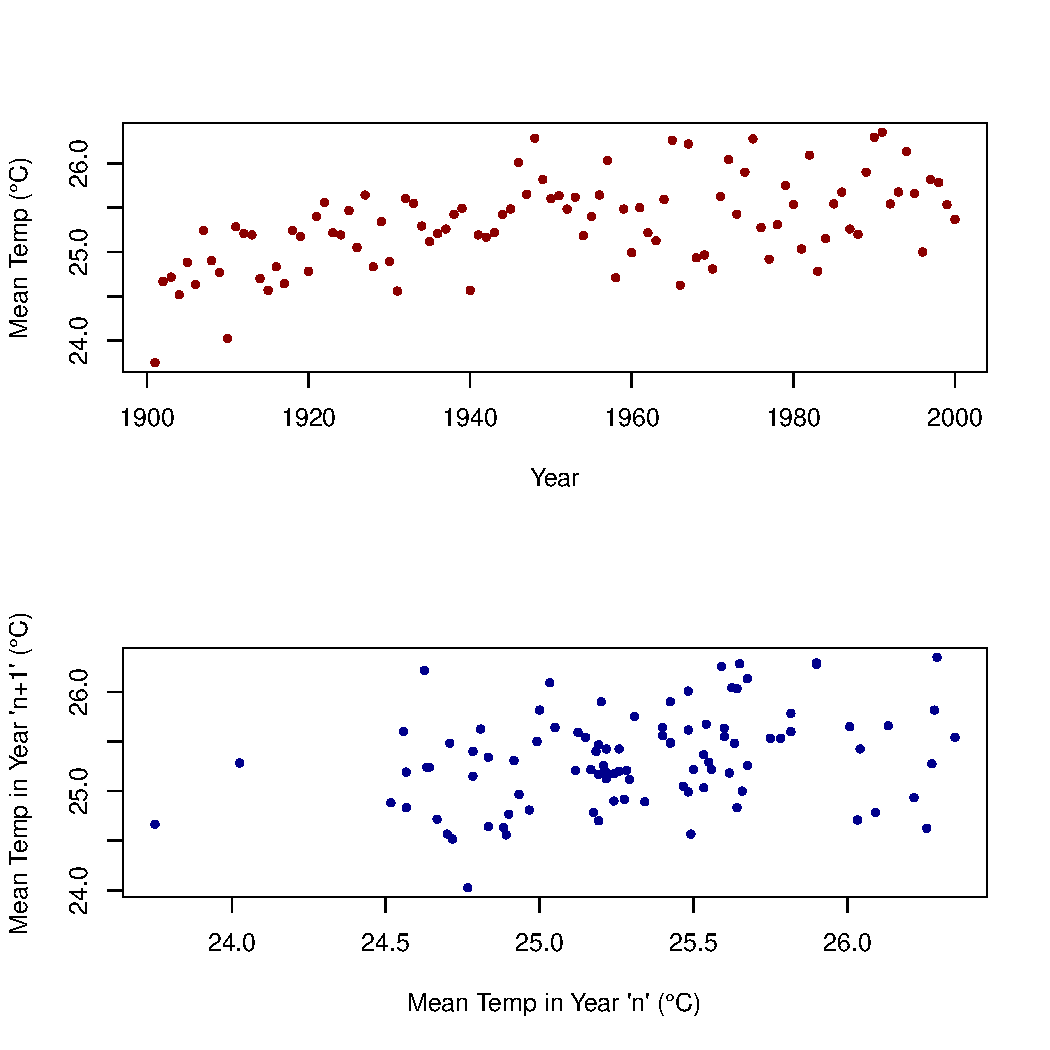
\includegraphics[width = 4in, height = 6in]{../data/ACC_Data.pdf}
\caption{A scatterplot showing the relationship between Temperatures 
(Degrees celcius) and Years at Key West, Florida.}
\label{fig:Fig1}
\end{figure}
    
\newpage
\section{Results}
The analysis calculates the correlation coefficient between successive 
years to be 0.326 (3 s.f.), which signifies that there is a slight 
positive correlation for temperatures between successive years.

\begin{figure}[hbt!]
\centering
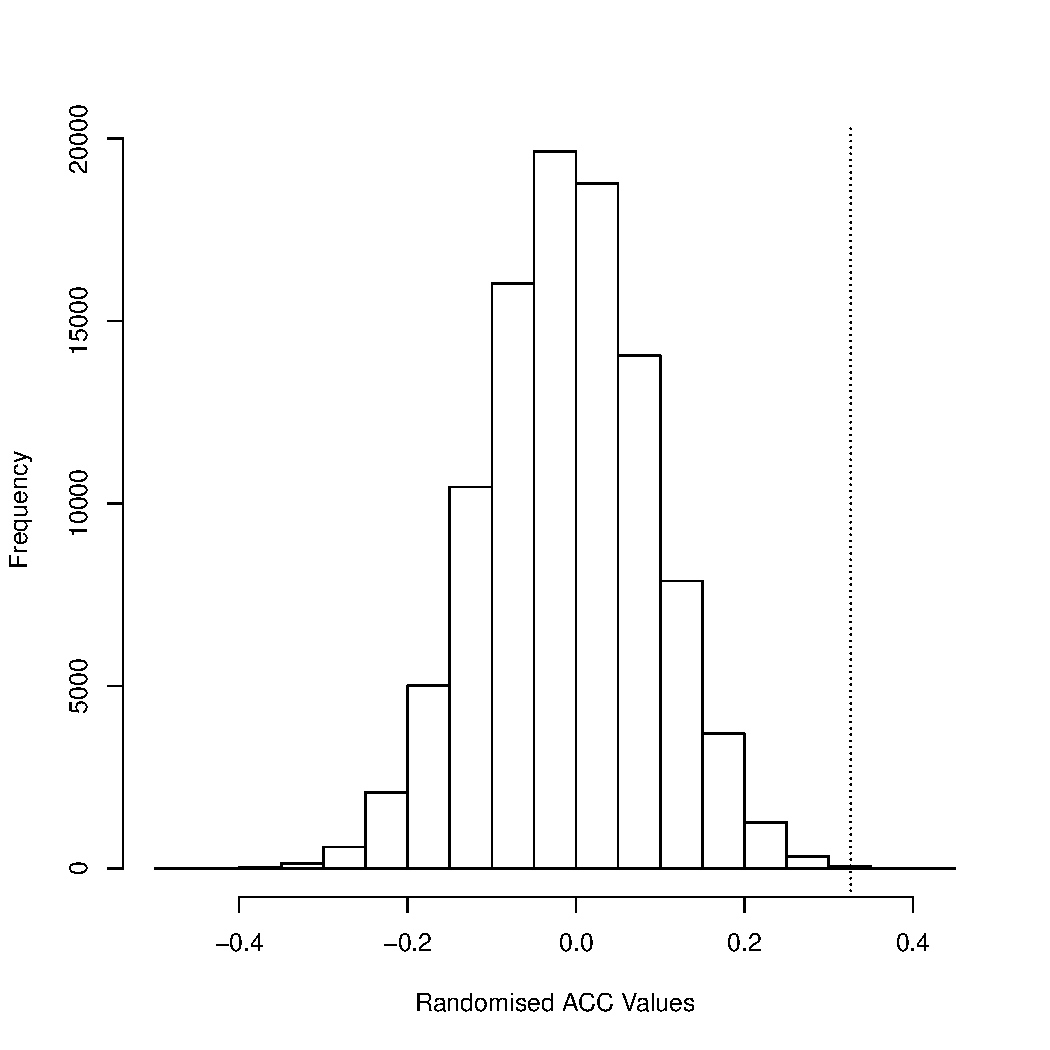
\includegraphics[width = 4in, height = 3in]{../data/ACC_Hist.pdf}
\caption{A histogram showing the distribution of correlation 
coefficients from randomly ordered temperatures.} 
\label{fig:Fig2}
\end{figure}

\newpage
Due to the random sampling, the p-value would fluctuate, however the 
seed had been set at 1 for reproducibility. The range of p-values 
obtained are much smaller than 0.05, which rejects the null hypothesis 
and accepts the alternative hypothesis where there is a strong 
significance in the correlation for temperatures between successive 
years. 

\end{document}